%%%%%%%%%%%%%%%%%%%%%%%%%%%%%%%%%%%%%%%%%%%%%%%%%%%
%% P3: Phenomenology of Particle Physics                         
%%
%% Author:  André Rubbia                   		 
%%
%% Figure 17.23 The ratio $2xF^{ep}_1/F_2^{ep}$ vs. $x$ for different $Q^2$ values (1.5 GeV$^2 < Q^2 < 16$ GeV$^2$).
%%
%% This work is licensed under the Creative Commons Attribution 4.0 International License. 
%% To view a copy of this license, visit http://creativecommons.org/licenses/by/4.0/ or 
%% send a letter to Creative Commons, PO Box 1866, Mountain View, CA 94042, USA.
%%
%%%%%%%%%%%%%%%%%%%%%%%%%%%%%%%%%%%%%%%%%%%%%%%%%%%

\documentclass[a4paper,10pt]{article}

\usepackage[T1]{fontenc}
\usepackage[utf8]{inputenc}
\usepackage{lmodern}
\usepackage[labelfont=bf]{caption}
\usepackage{upgreek}

\usepackage{tikz}
\usepackage{pgfplots}
\pgfplotsset{compat=1.17}
\usepgfplotslibrary{ternary}
\usepgfplotslibrary{fillbetween}
\usepgfplotslibrary{external}

\def\d{\mathrm{d}}

\begin{document}

%%%%%%%%%%%%%%%   FIGURE  %%%%%%%%%%%%%%%%%%%%%%%%%%%%%%
\begin{figure}[htb]
\begin{center}
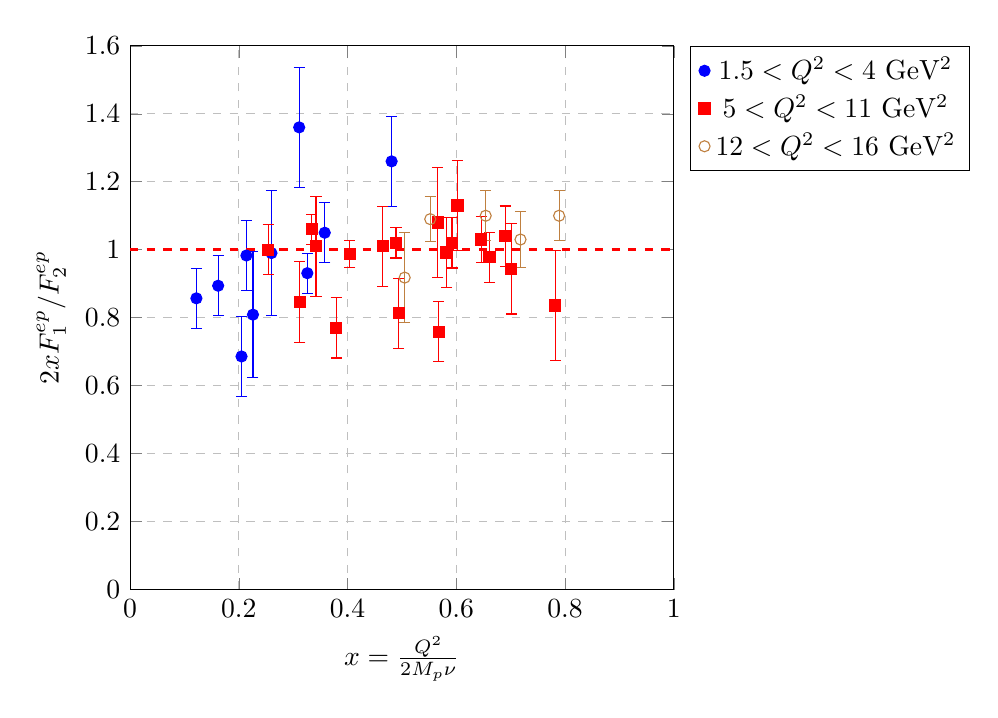
\begin{tikzpicture}[scale=1]
\begin{axis}[
width=0.7\textwidth,
height=0.7\textwidth,
    xlabel={$x=\frac{Q^2}{2M_p\nu}$},
    ylabel={$2xF^{ep}_1/F_2^{ep}$},
    xmin=0, xmax=1,
    ymin=0, ymax=1.6,
	legend style={legend pos = outer north east},
    	ymajorgrids=true,
    	xmajorgrids=true,
    grid style=dashed
]

    \addplot[
    color=blue,
    only marks, mark=*,
    error bars/.cd,
    y dir=both, y explicit
    ]
    coordinates {
    (0.122,0.857)+-(0,0.088669951)
    (0.162,0.89408867)+-(0,0.088669951)
    (0.205,0.686)+-(0,0.118226601)
    (0.214,0.983)+-(0,0.103448276)
    (0.226,0.809)+-(0,0.184729064)
    (0.260,0.990147783)+-(0,0.184729064)
    (0.311,1.36)+-(0,0.177339901)
    (0.326,0.931)+-(0,0.0591133)
    (0.358,1.05)+-(0,0.088669951)
    (0.481,1.26)+-(0,0.133004926)
    };

        \addplot[
    color=red,
    only marks, mark=square*,
    error bars/.cd,
    y dir=both, y explicit
    ]
    coordinates {
    (0.254,1.0)+-(0,0.073891626)
    (0.312,0.846)+-(0,0.118226601)
    (0.334,1.06)+-(0,0.044334975)
    (0.342,1.01)+-(0,0.147783251)
    (0.379,0.770)+-(0,0.088669951)
    (0.404,0.988)+-(0,0.04)
    (0.465,1.01)+-(0,0.118226601)
    (0.489,1.02)+-(0,0.044334975)
    (0.494,0.813)+-(0,0.103448276)
    (0.566,1.08)+-(0,0.162561576)
    (0.568,0.759)+-(0,0.088669951)
    (0.582,0.992)+-(0,0.103448276)
    (0.592,1.02)+-(0,0.073891626)
    (0.602,1.13)+-(0,0.133004926)
    (0.646,1.03)+-(0,0.066502463)
    (0.661,0.978)+-(0,0.073891626)
    (0.690,1.04)+-(0,0.088669951)
    (0.701,0.944)+-(0,0.133004926)
    (0.782,0.836)+-(0,0.162561576)
    };

    \addplot[
    color=brown,
    only marks, mark=o,
    error bars/.cd,
    y dir=both, y explicit
    ]
    coordinates {
    (0.505,0.918)+-(0,0.133004926)
    (0.552,1.09)+-(0,0.066502463)
    (0.654,1.10)+-(0,0.073891626)
    (0.718,1.03)+-(0,0.081280788)
    (0.789,1.10)+-(0,0.073891626)
    };

      \legend{$1.5<Q^2<4$~GeV$^2$,
     $5<Q^2<11$~GeV$^2$,
     $12<Q^2<16$~GeV$^2$
      };

      \draw[red,dashed,very thick] (axis cs:0,1) -- (axis cs:1,1);

\end{axis}
\end{tikzpicture}
\caption{The ratio $2xF^{ep}_1/F_2^{ep}$ vs. $x$,
for different $Q^2$ values (1.5 GeV$^2 < Q^2 < 16$ GeV$^2$). The data is from the
SLAC-MIT experiment described in Section~16.6 of the book.}
\end{center}
\end{figure}
%%%%%%%%%%%%%%%  END FIGURE  %%%%%%%%%%%%%%%%%%%%%%%%%%%%%%
%

\end{document}
